% LaTeX template for Artifact Evaluation V20180713
%
% Prepared by 
% * Grigori Fursin (cTuning foundation, France and dividiti, UK) 2014-2018
% * Bruce Childers (University of Pittsburgh, USA) 2014
%
% See example of this Artifact Appendix in
%  * SC'17 paper: https://dl.acm.org/citation.cfm?id=3126948
%  * CGO'17 paper: https://www.cl.cam.ac.uk/~sa614/papers/Software-Prefetching-CGO2017.pdf
%  * ACM ReQuEST-ASPLOS'18 paper: https://dl.acm.org/citation.cfm?doid=3229762.3229763
%
% (C)opyright 2014-2018
%
% CC BY 4.0 license
%

\documentclass[10pt,twocolumn,nocopyrightspace]{sigplanconf}

% preprint      Remove this option only once the paper is in final form.
% 10pt          To set in 10-point type instead of 9-point.
% 11pt          To set in 11-point type instead of 9-point.
% authoryear    To obtain author/year citation style instead of numeric.
\usepackage{fancyhdr}
\usepackage{amsmath}

%% BEGIN PREAMPLE
\usepackage{graphicx}
\usepackage{amsmath}
\usepackage{algorithm}
\usepackage{algorithmic}
\usepackage{amssymb}
\usepackage{url}
%% \usepackage[]{hyperref} %FOR CAMERA READY NO BOOKMARKS!

%% Tables
%\usepackage[table]{xcolor}


\title{Function Merging by Sequence Alignment}

\authorinfo{\text{Rodrigo Rocha, $\,$ Pavlos Petoumenos}}
           {University of Edinburgh, UK}
           {\url{r.rocha@ed.ac.uk}, \url{ppetoume@inf.ed.ac.uk}}

%\authorinfo{Rodrigo C. O. Rocha}
%           {University of Edinburgh, UK}
%           {\url{r.rocha@ed.ac.uk}}
%
%\authorinfo{Pavlos Petoumenos}
%           {University of Edinburgh, UK}
%           {\url{ppetoume@inf.ed.ac.uk}}
%
\authorinfo{Zheng Wang}
           {Lancaster University, UK}
           {\url{z.wang@lancaster.ac.uk}}
%
%\authorinfo{Murray Cole}
%           {University of Edinburgh, UK}
%           {\url{mic@inf.ed.ac.uk}}
%
%\authorinfo{Hugh Leather}
%           {University of Edinburgh, UK}
%           {\url{hleather@inf.ed.ac.uk}}

\authorinfo{Murray Cole, $\,$ Hugh Leather}
           {University of Edinburgh, UK}
           {\url{mic@inf.ed.ac.uk}, \url{hleather@inf.ed.ac.uk}}

%% END OF PREAMPLE
\begin{document}
\maketitle

\section{Introduction}
\label{sec:introduction}

In recent years, resource-constrained devices have become increasingly
important. Application binaries for these devices often reach several megabytes
in size, turning memory size into a limiting factor~\cite{plaza18}. Just adding more
memory is not always a viable option. Highly integrated systems-on-chip are
common in this market and their memories typically occupy the largest fraction
of the chip area, contributing to most of the overall cost. Even small
increases in memory area translate directly to equivalent increases in cost,
which lead to enormous levels of lost profit at large scales~\cite{edler10}.

In such constrained scenarios, reducing the code size is essential~\cite{sehgal12,keoh14,auler17}.
Unfortunately, production compilers offer little help beyond dead-code
elimination or merging identical functions~\cite{tallam10,kwan12,livska14}.
Developers might have more luck just removing functionality from their
libraries~\cite{keoh14} or hand-optimizing their code~\cite{weaver09}.

%Furthermore, the rise of the Internet of Things (IoT) depends heavily on tiny and efficient devices.
%Some of these devices can have as little as only a few kilobytes of
%memory~\cite{yelamarthi17,plaza18}.
%At the same time, low-end devices have been playing an important role in driving
%innovation in developing countries~\cite{hart02,etzo10}.
%As a result, there is an increasing focus on the development of programs
%tailored for these low-end devices with limited memory sizes~\cite{androidGo,hahm16}.

Function merging reduces replicated code by combining multiple identical
functions into a single one~\cite{llvm-fm,livska14}. 
Although a simple and intuitive concept, it is crucial for making high-level
abstractions usable, when they introduce duplicate code~\cite{tallam10,kwan12}.
For example, some C++ ABIs may end up creating multiple identical constructors
and destructors of a class to use in different contexts~\cite{kwan12} and C++
templates replicate code for different specializations~\cite{tallam10,livska14}.
More advanced approaches~\cite{edler14} have extended this idea into
merging non-identical functions by leveraging structural similarity. Functions
with identical control-flow graphs (CFGs) and only small differences within
corresponding basic blocks are merged into a single function that maintains
the semantics of the original functions. This is particularly important for
handling specialized template functions with small differences in their
compiled form.

While an improvement, even the state-of-the-art often usually fails to produce any
noticeable code size reduction. In this paper, we introduce a novel way to merge
functions that overcomes the major limitations of the state-of-the-art. Our
insight is that the weak results of existing function merging implementations
are not due to the lack of duplicate code but due to the rigid, overly restrictive
algorithms they use to find duplicates.

Our approach is based upon the concept of sequence alignment, developed in
bioinformatics for identifying functional or evolutionary relationships between
different DNA or RNA sequences. Similarly, we use sequence alignment to find
areas of functional similarity in arbitrary function pairs. Aligned segments
with equivalent code are merged. The remaining segments where the two functions
differ are added to the new function too but have their code guarded by a
function identifier. This approach leads to significant code size reduction.
%more than three times better than the state-of-the-art can achieve.

Applying sequence alignment to all pairs of functions is prohibitively expensive
even for medium sized programs. To counter this, our technique is integrated with
a ranking-based exploration mechanism that efficiently focuses the search to the most
promising pairs of functions. %\todo{whats interesting about this ranking?}.
As a result, we achieve our code size savings while introducing little compilation-time
overhead.

%Compared to identical function merging, we introduce extra code to be executed,
%namely the code that chooses between dissimilar sequences in merged functions.
%A naive implementation could easily hurt performance, e.g by merging two hot
%functions with only few similarities.
%Our technique can avoid this by incorporating profiling information to identify
%blocks of hot code and effectively minimize the overhead in this portion of the code.

In this work, we make the following contributions:
\begin{itemize}
  \item We are the first to allow merging arbitrary functions, even ones with
    different signatures and CFGs.
  \item A novel ranking mechanism for focusing inter-procedural optimizations
    to the most profitable function pairs.
  \item Our function merging by sequence alignment technique is able to reduce
     code size by up to 25\% on Intel and 30\% on ARM, significantly outperforming the
     state-of-the-art, while introducing minimal compile-time and negligible run-time overheads.
\end{itemize}

%In order to focus the optimization on promising pairs of functions,
%our technique is integrated with a ranking-based exploration mechanism.
%As a result, our optimization is more than three times better than the
%state-of-the-art for reducing code size with little compilation-time overhead.
%Our optimization is able to reduce size of the compiled programs by up to
%22\% over the already highly optimized baseline, with an average code-size
%reduction of about 5.6\%.
%These optimization can be carried on with little or no significant impact on
%performance, especially when aided by profiling information.
%Moreover, aided by profiling information, these optimization can be carried on
%without any significant impact on performance.
%We also propose a ranking-based exploration mechanism so that we can focus
%the optimization on promising pairs of functions.
%Our prototype introduces an average overhead of only 20\% in compilation time.



%Most of the classic optimizations try to find semantically equivalent programs
%that require fewer instructions to execute, such as dead code elimination,
%common subexpression elimination, and others~\cite{cocke70,massalin87,knoop94}.
%Although initially motivated by performance, these optimizations achieve better
%performance by focusing on code-size reduction.

%However, we distinguish the optimizations that focus on code-size reduction in
%two main categories:
%  (1) optimizations that find a smaller number instructions
%  that are required to execute in order to perform the same computation, e.g.,
%  common subexpression elimination, superoptimization, peephole optimization,
%  etc.~\cite{cocke70,massalin87,cooper99,tanenbaum82}.
%  (2) optimizations that change the representation of the same sequence of
%  instructions in a more compact manner, e.g., code compression, 
%  code factoring, function merging,
%  etc.~\cite{ernst97,debray00,chen03,loki04,edler14}.

%Code-size reduction is especially important for embedded or
%low-end devices~\cite{schultz03,varma04,sehgal12,keoh14,auler17}, as some
%of these devices can have only a few kilobytes of memory~\cite{plaza18}.

%However, even in high-end devices, on-chip memory is very limited in size, and
%if well utilized can result in good performance. 
%Moreover, there has been many attempts towards high-performance computation at
%low costs~\cite{phelan03}.


%For example, Android Go is a tailored Android distribution for low-end devices
%that has a major focus on code size reduction for both the operating system itself
%and the applications, suitable for devices with 1~GiB
%of RAM or less~\cite{androidGo}.

%However, we argue that even when storage and memory resources are abundant,
%compilers should ideally heavily optimize cold code for size reduction while
%optimizing hot code for performance.
%This idea is evident in many attempts, in both research and industry, of
%performing high-performance computation at low cost.

%\cite{weaver09}
%\cite{steenkiste89}
%\cite{zmily06}

%Differently from most of the optimizations that perform code-size
%reduction~\cite{cocke70,massalin87,cooper99}, which reduces the number of
%instructions that need to be \textit{executed} in order to perform the same
%computation, there are other optimizations that perform code-size
%reduction by reducing the number of instructions necessary to \textit{represent}
%the same computation.
%Note that in the second case, the actual number of instructions executed
%may not differ or, sometimes, even increase.
%One such optimization is function merging, which 


\section{Our Approach} \label{sec:fm}

%% I don't think the compilation pipeline should be here.
%% The optimization does not need to be performed during link-time.
%% I think it is part of our experimental setup, that's way it was in the result section.
%% It could be performed per compilation-unit as well.
%\begin{figure}[t!]
%  \centering
%  \includegraphics[width=0.7\linewidth]{figs/opt-pipeline.pdf}
%  \caption{The compilation pipeline of our approach.}
%  \label{fig:opt-pipeline}
%\end{figure}

%\subsection{The Compilation Pipeline}
%Our approach is implemented as an LLVM pass to perform at the LLVM IR level. Therefore, it can perform function merging across application
%and library code.

%Figure~\ref{fig:opt-pipeline} shows an overview of the compilation pipeline using our function merging (FM) approach. First, we apply early
%code-size optimizations per compilation-unit (e.g., \update{functions and basic blocks}). Then, function merging and further code-size
%optimizations are applied during monolithic link-time optimization~(LTO). With LTO, object file generation is delayed until all input
%modules are known, instead of being generated per
%compilation-unit, which enables more powerful optimizations based on whole-program analyses. %The baseline uses exactly the same compilation
%%%%pipeline, except for not having any function-merging optimization.

Intuitively, when we are manually merging two functions, in a textual format, we try to visualize them side by side, identifying the
equivalent segments of code and the non-equivalent ones. Then, we use this understanding to create the merged function. In this paper, we
propose a technique that follows this simple yet effective principle. At the core of our technique lies a sequence alignment algorithm,
which is responsible for arranging the code in segments that are either equivalent or non-equivalent.
We implement this technique at the level of the intermediate representation (IR).
Our current implementation assumes that the input functions have all their $\phi$-functions demoted to memory operations,
simplifying our code generation.

\begin{figure}[t!]
  \centering
  \includegraphics[width=0.85\linewidth]{figs/func-merge-overview.pdf}
  \caption{Overview of our function-merging technique.
           Equivalent segments of code is represented in light green and the non-equivalent ones in dark red.}
  \vspace{-1em}
  \label{fig:func-merge-overview}
\end{figure}

The proposed technique consists of three major steps, as depicted in
Figure~\ref{fig:func-merge-overview}.
First, we linearize each function, representing the CFG as a sequence of
labels and instructions.
The second step consists of applying a sequence alignment algorithm, borrowed
from bioinformatics, which identifies regions of similarity between sequences.
The sequence alignment algorithm allows us to arrange two linearized functions
into segments that are equivalent between the two functions and segments where
they differ from one another.
The final step performs the code generation, actually merging the two functions.
Aligned segments with equivalent code are merged, avoiding redundancy,
while the remaining segments where the two functions differ have their code
guarded by a function identifier.

During code generation, we create a merged list of parameters, including the
extra function identifier if there are any dissimilar segments. 
Arguments of the same type are shared between the functions, without necessarily
keeping their original order.
We also allow for the return types to be different, in which case we use an
aggregate type to return values of both types.
If one of them is void, then we do not create an aggregate type, we just return the non-void type.
Given the appropriate function identifier, the merged function is semantically equivalent to the original functions,
so we replace all of their invocations with the new function.
It should be noted that in the special case where we merge identical functions, the output is also identical, emulating
the behavior of function merging in production compilers.

After producing the merged function, the bodies of the original functions are
replaced by a single call to this new function, creating what is sometimes
called a \textit{thunk}.
In some cases, it may also be valid and profitable to completely delete the
original functions, remapping all their original calls to the merged function.  
Two of the key facts that prohibit the complete removal of the original functions
are the existence of indirect calls or the possibility of external linkage.


Our technique works on any two arbitrary functions, even when they have few
similarities and merging them would
be counter-productive. For that reason, we also introduce a cost model to decide
when it is beneficial to merge two functions.
To avoid an expensive quadratic exploration, we integrate our profitability analysis
with an efficient ranking mechanism based on a lightweight fingerprint of the functions.


After generating the code of the merged function, we need to estimate the
code-size benefit of replacing the original pair of functions by the new merged
function.
In order to estimate the code-size benefit, we first compute the code-size cost
for each instruction in all three functions.
In addition to measuring the difference in size of the merged function, we also
need to take into account all extra costs involved:
$(1)$ for the cases where we need to keep the original functions with a call to
the merged function;
and $(2)$ for the cases where we update the call graph, there might be an extra
cost with a call to the merged function due to the increased number of arguments.
 

\bibliographystyle{abbrvnat}
\bibliography{bib/refs}
\end{document}
